%!TEX root = /Users/Abj/git/MiL/report/report.tex
\part{Solutions}
%As the previous sections of the \texttt{In-depth phase} in part \ref{prt:in_depth_analysis},
%especially in section \ref{sub:goprne}, has shown,
%the organisation has room for optimisation and improvements. Based on the \ref{sub:ideas} that we
%have developed and the fact that the organisation wants to continue using Podio, we have chosen two that we believe will bring the most benefits to the organisation.
%We will in the following analyse both the solutions, and try to determine which will be the best or
%if a third solution will emerge from this analysis. A short description of the ideas in focus
%follows:


%1. Work processes for Podio\\
%In the previous the Diagnostic Map in section xx revealed several problem and related causes found in the organization. In 5b its said that the cause of this problem, is that their is too much off topic discussion and also that no real difference between pure informational topics and topics for discussions are in place within the organizational use of Podio. As Stine F also points out in 1a, the organization faces a problem about sharing of knowledge, since this is not documented properly on Podio.\\

%This solution proposal will attempt to structure work processes when using Podio and make guidelines for the information posted at Podio. This proposal will therefore be  directed at the use of Podio, with respect to the mentioned things in the above, and will keep to the organizations strategy about using Podio as their primary IT solution. 

%2. Podio App
%This solution consists of the development of a Podio application \footnote{https://developers.podio.com/doc/app-store}.
%The application will be used to create, store, and visualise tasks in- and externally in the teams.
%Thus, hopefully, making it very transparent which tasks are due to when.\\





  
\section{Solution 1 - Podio Guidelines}

\subsection{Vision for overall change} 
This presented solution is a minimalistic approach, designed to extend the current work flow of the
arrangers. The goal of it is to introduce procedures to keep the communication flow of Podio clean.
With the current usage of Podio, it takes advantage of user's existing level of knowledge of the
platform, by not introducing new artifacts, but merely moving and defining domains and corresponding procedures. Specifically this solution seeks to introduce the following ideas:

\begin{itemize}
    \item An informal podio-space for unrelated communication between all MiL members. Topics unrelated to the planning of MiL are posted to this space to keep important information or decisions visible in the remaining workspaces.
    \item Guidelines for Podio:
    \begin{enumerate}
        \item Questions or information of significance to organising the festival are posted to
        their appropriate workspaces. This means a status regarding booking of urinals should be
        posted to the festival area-space, while general information such as a new booked musical
        act are posted to the employee space. Remaining content such as music acts on other
        festivals are referred to the previously mentioned "informal space".
        \item Questions with expected results, e.g. non-discussional, should not be posted as posts but created as a podio task with a specified deadline. 
        \item All meetings are documented through the podio calendar app. They are created on
        beforehand with its agenda and updated with a minute containing the matters discussed at the
        meeting, this includes discussions and decisions agreed upon.
        \item Ad-hoc decisions are added to the next occurring meetings agenda. This insures that
        information does not disappear or becomes bound to single members, unobtainable for others.
    \end{enumerate}
    \item Appointed moderators to maintain the content of the workspaces to ensure that the specified guidelines are met.
\end{itemize}

\subsection{Technology}
The solution is based on the existing web application, Podio. Though having extensive access to customizable apps and library settings, this solution takes use of the standard utilities that are already being used by MiL. Overall this solution maintains the level of complexity by avoiding adding new artifacts to the work domain.

\subsubsection{User interfaces}
Since this solution does not add any new functionality to Podio, we do not really see any reason to
explain the user interface of this solution. The users are used to the Podio user interface, which
is a good thing, since the new the users does not have to get used to a new looking system.

\subsection{Work organisation}
Due to this solution remaining within the current domain of used technologies, the real introduction of change, appears in the work practices of members of MiL. Arrangers and teamleaders will be forced to adjust there work rutines in compliance to the previously stated guidelines, effectively inflicting their work flow. 
This specifically means that arrangers and teamleaders must take active actions to create tasks, and be aware of where content is posted while newly appointed moderators will hafto take on additional responsibility of maintaining the content podio spaces.

\subsection{Qualification needs}
As this solution is based on the Podio platform and its basic features, teamerleaders and the remainder of arrangers are required to have knowledge of how to use podio.  

\subsection{Advantages and disadvantages}
\begin{center}
    \begin{tabular}{ | p{7cm} | p{7cm} |}
    \hline
    \textbf{Advantages} & \textbf{Disadvantages}  \\ \hline
    Cleans the content of spaces and removes drowning of information & Misinterpretation of procedures, leading to unuseful content on Podio  \\ \hline
    Information is easy to find & Conflicts with MiLs informel approach to communication \\
    \hline
    Introduces structure to the way MiL uses podio & Members of MiL limit their use of podio \\ \hline
    \end{tabular}
\end{center}

\subsection{Finances}
The figure below shows the cost benefit analysis of this solution. The details can be found in [\ref{sec:cost_benefit_analysis}].
\begin{figure}[h!]
  \centering
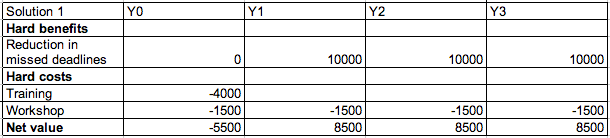
\includegraphics[scale=0.5]{Pictures/cost-benefit1.png}
    \caption{Cost benefit of Podio Work processes (units in DKK)}
\end{figure}

\subsection{Implementation strategy and plan} 
The most appropriate way to implement this solution is to introduce it as a pilot project. The initial target group would be the communication groups space, due to their high activity on Podio. By doing so, the solution is exposed early on and provides experience towards potential adjustments.

\section{Solution 2 - Podio extension}
\subsection{Visions for change}
\label{visions_for_change}
This solution is at its heart an interactive visualization of tasks and task dependencies across arranger teams. Tasks are communicated between arranger teams with the already present infrastructure present in Podio. The task window however, is extended with the following functionality and data:
\begin{itemize}
    \item Tasks can include subtasks. Subtasks are added to a task by pressing the "Add Subtask" button. When teams assign tasks to other teams, the receiving team may choose to define subtasks, that need to be completed before the assigned task can be completed. Subtasks can either be already existing tasks, or new tasks.
    \item Tasks include a "Done" description, in which the sender of the task may include a short description of when the task is considered to be done.
    \item Tasks are done when the receiving team presses the "Done" button under a task.
\end{itemize}
The data and functionality described above makes it possible to create a task map. The task map displays all active tasks in the system. A task is active if any of its subtasks are incomplete, or if it is itself a subtask to a task that is incomplete. Tasks are displayed graphically, with dependencies between them drawn as an directed arrow between them. Clicking a task will take the user to the task on Podio, where a detailed view of the task can be found. 
\\ \\
This solution will give arrangers an overview of deadlines, tasks associated with deadlines and dependencies between them across arranger teams, as to address problems discussed in (ref diagnostic map). By extracting deadline information and placing it collectively in the task map, confusion about where to find information about deadlines is reduced.


\subsection{Technology}
\label{sub:technology}
The solution uses the built in functionality of Podio to build custom Podio apps to create the needed modifications to Podio tasks. The task map is drawn on a webpage outside of the Podio domain, using the Podio REST API.

\subsubsection{IT systems and IT platform}
The solution is primarily dependent on the existing Podio platform. It is necessary that Podio maintains the possibility of defining custom apps and accessing Podio data through the REST API.

\subsubsection{User interfaces}
On Podio, the interface is built using the existing Podio app builder tools. The task map is displayed by some Web UI technology. Tasks are shown as nodes, and dependencies between them are shown as directed arrows. Task completion status is indicated graphically by color. (ref til mock up)

\subsection{Work organisation}
\label{sub:work_organisation}
Arrangers and team leaders will have to change their work-flow with creating tasks, to comply with the format described in section \ref{visions_for_change}. An introduction to using the task map must also be created. Some teams already use tasks (ref til podio analyse), and others do not. The teams that are not familiar with tasks will have to be introduced to them, and some encouragement and reinforcement is likely to be necessary.

\subsection{Qualification needs}
\label{sub:qualification_needs}
The solution depends on arrangers and team leaders using Podio correctly. This means that arrangers and team leaders must know how to use Podio.

\subsection{Advantages and disadvantages}
\label{sec:advantages_disadvantages}
\begin{center}
    \begin{tabular}{ | p{7cm} | p{7cm} |}
    \hline
    \textbf{Advantages} & \textbf{Disadvantages}  \\ \hline
     Raises awareness of deadlines and dependencies between teams & Risk of arrangers not using the system\\ \hline
     Makes information about deadlines easier to find & Time must be invested in teaching arrangers how to and when to create tasks\\ \hline
     Integrated with a system that is already known and used by arrangers and team leaders & Solution is dependent on Podio maintaining custom app possibilities and a Web service interface \\ \hline
    \hline
    \end{tabular}
\end{center}


\subsection{Finances}
The figure below shows the cost benefit analysis of this solution. The details can be found in [\ref{sec:cost_benefit_analysis}].
\begin{figure}[h!]
  \centering
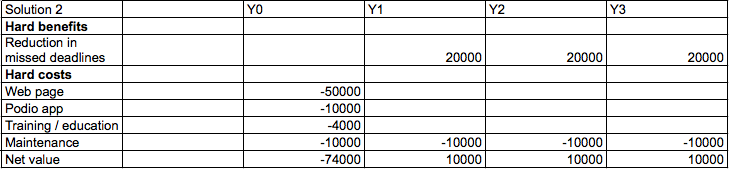
\includegraphics[scale=0.5]{Pictures/cost-benefit2.png}
    \caption{Cost benefit of Podio extension (units in DKK)}
\end{figure}

\subsection{Implementation strategy}
The pilot project strategy is recommended for this solution. Potential short comings and problems can be corrected before trying it with the whole organization. The bar team, fetival site team and volunteer team are good candidates for pilot teams, as significant dependencies exist between them (ref til stine interview eller flowchart).

A possible challege when implementing the strategy is motivating arrangers and team leaders to assign tasks on Podio, instead of sending messages or posting on walls of other groups etc. One strategy is to demonstrate the value of the task map, and how the usefulness of this tool is increased for everyone, when more arrangers use the task feature of Podio.

\section{Prioritization of solutions}
As argued in [\ref{sec:cost_benefit_analysis}] some assumptions about numbers of deadlines missed have been made. It is however still possible to make a prioritization of the suggested solutions.
The mentioned advantages and disadvantages for both solutions is possible to compare. The impact of solution 2, in terms of the reduced number of deadlines, is greater [\ref{sec:cost_benefit_analysis}]. However, as a consequence of the cost of solution 2, making the investment in this solution will not break even until the end of year 2 after making the ivestment. In comparison, solution 1 will break even after less than 1 year.
\\ \\
In terms of risk, solution 2 is dependent on some features offered by Podio, where as solution 1 is merely dependent on adaption from the arrangers and team leaders. In other words, solution 2 depends on some external factors, that are outside of the control of Musik i Lejet, where as the guidelines poroposed by solution 1, relies solely on Musik i Lejet's willingness to embrace the solution. For this reason, the risk of solution 2 is estimated to be more significant.
\\ \\
Based on these arguments, it is recommended that Musik i Lejet invests in solution 1. 


